\documentclass[12pt]{article}
\usepackage{graphicx}
%\documentclass[journal,12pt,twocolumn]{IEEEtran}
\usepackage[none]{hyphenat}
\usepackage{graphicx}
\usepackage{listings}
\usepackage[english]{babel}
\usepackage{graphicx}
\usepackage{caption} 
\usepackage{hyperref}
\usepackage{booktabs}
\usepackage{commath}
\usepackage{gensymb}
\usepackage{array}
\usepackage{amsmath}   % for having text in math mode
\usepackage{listings}
\lstset{
  frame=single,
  breaklines=true
}
  
%Following 2 lines were added to remove the blank page at the beginning
\usepackage{atbegshi}% http://ctan.org/pkg/atbegshi
\AtBeginDocument{\AtBeginShipoutNext{\AtBeginShipoutDiscard}}
%


%New macro definitions
\newcommand{\mydet}[1]{\ensuremath{\begin{vmatrix}#1\end{vmatrix}}}
\providecommand{\brak}[1]{\ensuremath{\left(#1\right)}}
\providecommand{\norm}[1]{\left\lVert#1\right\rVert}
\newcommand{\solution}{\noindent \textbf{Solution: }}
\newcommand{\myvec}[1]{\ensuremath{\begin{pmatrix}#1\end{pmatrix}}}
\let\vec\mathbf
\begin{document}
\begin{center}
\title{\textbf{Circles}}
\date{\vspace{-5ex}} %Not to print date automatically
\maketitle
\end{center}
\setcounter{page}{1}
\section{11$^{th}$ Maths - Exercise 11.1.8}

\begin{enumerate}
\item Find the centre and radius of the given circle $\vec{x}^2+\vec{y}^2-8\vec{x}+10\vec{y}-12=0$
\section{Solution}
The general equation of  the circle is 
\begin{align}
\norm{\vec{x}}^{2} + 2\vec{u}^{\top}\vec{x} + f = 0
\end{align}
by using above equation
\begin{align}
	x^2+y^2-8x+10y-12=0\\
	\norm{\vec{x}}^2+2\myvec{-4 & 5}\vec{x}-12&=0
\end{align}	
Where,
\begin{align}
	\vec{u} &= -\vec{c} \text{ and } f = \norm{\vec{u}}^{2} - r^{2}\
\end{align}
\begin{align}
 \vec{u}&=\myvec{-4\\5}\\
 f&=-12\\
\vec{c}&=\myvec{4 \\ -5}\\
r^2&=\norm{\vec{u}}^2-f\\
r^2&= 53\\
r&=\sqrt{53}
\end{align}
\begin{figure}[!h]
	\begin{center} 
	   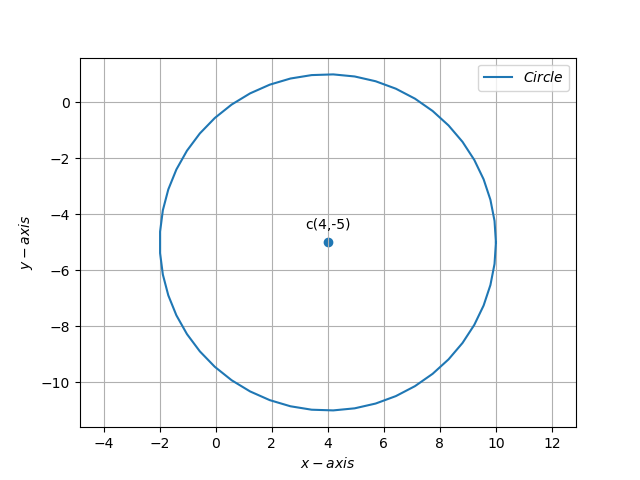
\includegraphics[width=\columnwidth]{figs/11.1.8.png}
	\end{center}
\caption{}
\label{fig:Fig1}
\end{figure}
\end{enumerate}
\end{document}